\chapter{Generalizing Newtonian Cosmology}

This lecture begins, characteristically, by stepping back before stepping forward. Before generalizing the Newtonian cosmology of the previous lecture, Susskind asks why Newton's equations were legitimate in the first place in a universe whose real description belongs to Einstein. Once that permission is granted, we review the moving-grid bookkeeping and the matter-only law \(a\propto t^{2/3}\). Then the lecture opens out in two directions. First, we back away from the knife-edge assumption of zero total energy and recover the extra \(a^{-2}\) term in the Friedmann equation. Second, we replace slowly moving matter by radiation, discover the scaling \(\rho_r\propto a^{-4}\), and arrive at the old but still fundamental two-component cosmology: radiation first, matter later, with dark energy still waiting offstage.

\section{Newton In A Curved Universe}

The lecture does not open with a derivation. It opens with a challenge: does Newton really get it right?

Einstein's equations describe curved spacetime, and perhaps curved space itself. A universe may be globally curved even if, over the region we currently observe, it looks nearly flat. Susskind's point is that this does not invalidate the Newtonian treatment we have been using. A sufficiently small patch of a curved space looks flat. If we restrict attention to the local behavior of neighboring galaxies, then the curvature of the full universe need not yet concern us.

This ``small patch'' can still be enormous by ordinary standards. It can mean a region much smaller than the radius of curvature of the universe, yet still billions of light-years across. What matters is not human scale but comparison with the curvature scale. On that local patch, Newtonian reasoning is consistent with Einstein.

There is only one important warning. The approximation fails if neighboring matter moves relativistically with respect to itself. Up to now we have deliberately stayed away from that regime. We have studied a comoving patch whose nearby contents move slowly enough for Newton to be reliable. But the universe is not filled only with slowly moving matter. It is also filled with radiation, and radiation moves at the speed of light. That is the opening signal for tonight's generalizations.

\section{Recap Of The Moving Grid And Matter-Only Expansion}

Let us recall the bookkeeping before we change the physics.

We imagine a homogeneous distribution of galaxies and lay down a comoving grid on it. If \(x\) is the comoving coordinate, then the physical distance between \(x\) and \(x+1\) is \(a(t)\). The important point is that \(a(t)\) itself is not yet an absolute observable. If we had chosen a coarser grid, every value of \(a\) would be larger by a fixed factor; with a finer grid, every value would be smaller.

What survives that ambiguity are ratios. If we rescale the grid by a constant factor \(\alpha\), then
\begin{align}
a' &= \alpha a, &
\dot a' &= \alpha \dot a,
\end{align}
so
\begin{equation}
\frac{\dot a'}{a'}=\frac{\dot a}{a}.
\end{equation}
That ratio is invariant under a once-and-for-all change of grid spacing. It is therefore physically meaningful. We call it the Hubble parameter,
\begin{equation}
H(t)\equiv \frac{\dot a}{a}.
\end{equation}

The same bookkeeping issue appears in \(\nu\), the amount of matter in one comoving unit cube. Its numerical value depends on the chosen grid, but once the grid is fixed it is constant in time for ordinary matter, provided matter is neither created nor destroyed. The physical density is then
\begin{equation}
\rho_m=\frac{\nu}{a^3}.
\end{equation}
The box grows, the matter in it stays the same, and so the density falls like \(a^{-3}\).

Real galaxies, of course, have peculiar motions on top of this average Hubble flow. The lecture explicitly sets those aside. The Friedmann equations describe the averaged motion, not the local orbital clutter superposed on it.

With that in place, we return to the matter-only, zero-energy equation derived in the previous lecture:
\begin{equation}
\left(\frac{\dot a}{a}\right)^2=\frac{8\pi G}{3}\rho_m
=\frac{8\pi G}{3}\frac{\nu}{a^3}.
\end{equation}
Because the grid normalization is arbitrary, and because changing the grid changes \(\nu\), we may choose the grid so that
\begin{equation}
\frac{8\pi G\nu}{3}=1.
\end{equation}
Then the equation simplifies to
\begin{equation}
\left(\frac{\dot a}{a}\right)^2=\frac{1}{a^3}.
\end{equation}

Now we solve it exactly as the lecture does. Taking a square root gives
\begin{equation}
\frac{\dot a}{a}=\pm \frac{1}{a^{3/2}},
\end{equation}
hence
\begin{equation}
\dot a=\pm \frac{1}{\sqrt a}.
\end{equation}
On a monotonic branch we invert the derivative and regard time as a function of \(a\):
\begin{equation}
\frac{dt}{da}=\pm \sqrt a.
\end{equation}
Integrating,
\begin{equation}
t=\pm \frac{2}{3}a^{3/2}+\text{const},
\end{equation}
and therefore
\begin{equation}
a(t)\propto t^{2/3}.
\end{equation}

This is the matter-dominated, zero-energy universe. It expands forever, but it decelerates. The graph of \(a(t)\) gets flatter and flatter. Yet it never truly stops, because the right-hand side of the differential equation becomes small but never vanishes.

The board at this stage is a recap board rather than a fresh derivation, and it is useful precisely for that reason: it records the solved matter-only case as a point of departure.

\begin{figure}
\centering

\includegraphics[width=0.62\textwidth]{lecture_02_figure_02.png}
\caption{Board recap of the matter-only solution, including \(\dot a=1/\sqrt a\) and the boxed \(a\sim t^{2/3}\) law.}
\end{figure}

At this point Susskind announces the two directions in which he wants to generalize the story. One is to abandon the arbitrary assumption of zero total energy. The other is to replace slowly moving matter by radiation. He takes the first one first.

\subsection{Question \& Answer}

Why are we allowed to discard the negative square root when solving the matter-only equation?

We are not allowed to discard it as a matter of mathematics. We discard it only after choosing a physical branch. The equation determines \((\dot a/a)^2\), and from that alone one cannot tell whether the universe is expanding or contracting.

Susskind answers with a simple Newtonian analogy. A rock moving radially in the field of a planet may be going out or coming in. Newton's equation does not say which. It only says what the acceleration is. The same is true here. The positive root describes an expanding branch, the negative root a contracting one. In the recap calculation we choose the expanding branch because that is the case under discussion, not because the equation itself ruled out contraction.

\section{Non-Zero Energy And The Extra Friedmann Term}

Now we go back to the energy equation and remove the knife-edge assumption that every galaxy is exactly at escape velocity.

We smooth the matter distribution, choose ourselves as the center, and use Newton's theorem: for a galaxy at comoving position \(x\), only the mass inside the sphere of radius \(D=ax\) matters dynamically. Everything outside the sphere can be ignored. The lecture then simplifies the discussion by choosing the particular galaxy with
\begin{equation}
x=1.
\end{equation}
For that galaxy,
\begin{equation}
D=ax=a,
\qquad
\dot D=\dot a\,x=\dot a.
\end{equation}

The board at this point shows the sphere, the central concentrated mass \(M\), the radial distance \(a\), and the label \(x=1\). It also uses the symbol \(V\) both for volume and for velocity. To avoid that ambiguity we will write \(V_{\text{sphere}}\) for the sphere's volume and \(\dot D\) for the radial velocity.

\begin{figure}
\centering

\includegraphics[width=0.82\textwidth]{lecture_02_figure_03.png}
\caption{Newtonian enclosed-mass construction and the non-zero-energy Friedmann equation on the board.}
\end{figure}

\begin{figure}
\centering
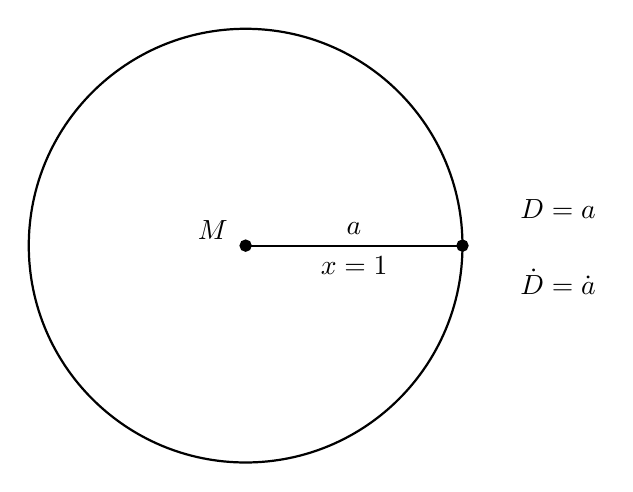
\begin{tikzpicture}[scale=1.02]
\draw[thick] (0,0) circle (2.7);
\filldraw (0,0) circle (2pt);
\node[left] at (-0.10,0.20) {$M$};
\draw[thick] (0,0)--(2.7,0);
\filldraw (2.7,0) circle (2pt);
\node[above] at (1.35,0.02) {$a$};
\node[below] at (1.35,-0.02) {$x=1$};
\node[right] at (3.30,0.45) {$D=a$};
\node[right] at (3.30,-0.45) {$\dot D=\dot a$};
\end{tikzpicture}
\caption{Clean reconstruction of the \(x=1\) enclosed-mass picture used in the Newtonian derivation.}
\end{figure}

The energy of the test galaxy is
\begin{equation}
\frac{1}{2}m\dot D^{\,2}-\frac{GMm}{D}=E.
\end{equation}
For the \(x=1\) galaxy, this becomes
\begin{equation}
\frac{1}{2}m\dot a^{\,2}-\frac{GMm}{a}=E.
\end{equation}
Divide by \(m\), multiply by \(2\), and absorb the resulting constant on the right into a new constant \(C\):
\begin{equation}
\dot a^{\,2}-\frac{2GM}{a}=C.
\end{equation}
Now divide by \(a^2\):
\begin{equation}
\left(\frac{\dot a}{a}\right)^2-\frac{2GM}{a^3}=\frac{C}{a^2}.
\end{equation}
For the sphere of radius \(a\),
\begin{equation}
V_{\text{sphere}}=\frac{4\pi}{3}a^3,
\qquad
M=\rho_m\,V_{\text{sphere}}=\rho_m \frac{4\pi}{3}a^3.
\end{equation}
Substituting this gives the non-zero-energy Friedmann equation,
\begin{equation}
\left(\frac{\dot a}{a}\right)^2-\frac{8\pi G}{3}\rho_m=\frac{C}{a^2}.
\end{equation}
Equivalently,
\begin{equation}
\left(\frac{\dot a}{a}\right)^2=\frac{8\pi G}{3}\rho_m+\frac{C}{a^2}.
\end{equation}

The central term on the board is partly hidden by Susskind's hand, so this is a transcript-guided reconstruction of the standard form rather than a literal pixel reading. But it is exactly the equation he is talking through.

The lecture does not press on to a closed-form solution. Instead it asks what the equation does at small \(a\) and at large \(a\).

At early times, when \(a\) is small, the matter term \(a^{-3}\) dominates the new term \(a^{-2}\). So the early expansion is unchanged:
\begin{equation}
a(t)\propto t^{2/3}
\qquad
(a \ \text{small}).
\end{equation}

For \(C>0\), the late-time story changes. As \(a\) grows, \(a^{-2}\) eventually dominates \(a^{-3}\), so
\begin{equation}
\left(\frac{\dot a}{a}\right)^2 \sim \frac{C}{a^2}.
\end{equation}
Taking the expanding branch,
\begin{equation}
\dot a \sim \sqrt{C},
\end{equation}
and hence
\begin{equation}
a(t)\propto t.
\end{equation}
The Newtonian analogy is exactly the one used in the lecture: throw an apple harder than escape velocity, and far from the gravitating body it simply coasts with nearly constant speed.

For \(C<0\), write \(C=-|C|\). Then
\begin{equation}
\left(\frac{\dot a}{a}\right)^2
=
\frac{8\pi G}{3}\frac{\nu}{a^3}
-
\frac{|C|}{a^2}.
\end{equation}
At small \(a\), the first term still dominates. But at sufficiently large \(a\), the negative \(a^{-2}\) term catches up. The right-hand side can then reach zero at a finite value of \(a\). That is the turning point: the expansion stops, and afterward the solution returns along the negative square-root branch.

Thus the matter-only universe admits three qualitatively distinct cases: zero energy, positive energy, and negative energy.

\subsection{Question \& Answer}

How can recollapse occur if \(\left(\dot a/a\right)^2\) is always nonnegative?

This is one of the lecture's best clarifying moments. The student objection is exactly right up to a point: the right-hand side can never become negative, because it is equal to a square. But it can become zero.

If we begin on the expanding branch, then \(\dot a>0\) initially. The only way the universe can ever begin contracting is by first passing through \(\dot a=0\). That is precisely what happens in the negative-energy case. The right-hand side remains nonnegative, reaches zero at a maximum size, and then the solution continues with the negative root:
\begin{equation}
\frac{\dot a}{a}=-\sqrt{\frac{8\pi G}{3}\frac{\nu}{a^3}-\frac{|C|}{a^2}}.
\end{equation}
The square never becomes negative. The branch changes.

\section{Geometry On The Left, Energy On The Right}

At this stage the lecture changes its tone. The same equation is now reread, not merely as a Newtonian energy balance, but as the one-component shadow of Einstein's equation.

Move the \(a^{-2}\) term to the left-hand side:
\begin{equation}
\left(\frac{\dot a}{a}\right)^2+\frac{C}{a^2}=\frac{8\pi G}{3}\rho.
\end{equation}
This is the board arrangement that Susskind emphasizes when he says: geometry on the left, source on the right.

\begin{figure}
\centering

\includegraphics[width=0.72\textwidth]{lecture_02_figure_04.png}
\caption{Board arrangement of Friedmann's equation as geometry on the left and source on the right.}
\end{figure}

The left-hand side is geometric. It contains the expansion rate, and the lecture announces that the extra \(a^{-2}\) term will next time be reinterpreted as spatial curvature. The right-hand side is the source: whatever energy and momentum fill the universe.

At precisely this point the Newtonian meaning of \(\rho\) must be upgraded. In the Newtonian derivation \(\rho\) was a mass density. In the relativistic reading it is total energy density. Setting the speed of light to one, we simply replace ``mass density'' by ``energy density.'' Rest mass contributes, but so do radiation and any other form of energy.

To make contact with the usual curvature notation, let us define
\begin{equation}
\kappa \equiv -C.
\end{equation}
Then the same equation becomes
\begin{equation}
\left(\frac{\dot a}{a}\right)^2-\frac{\kappa}{a^2}=\frac{8\pi G}{3}\rho.
\end{equation}
The board writes \(K\) at one stage and the lecture says \(\kappa\) a moment later; the point is the same. What was the raw Newtonian energy constant now becomes a curvature-style term.

For ordinary matter, substituting \(\rho=\nu/a^3\) gives
\begin{equation}
\left(\frac{\dot a}{a}\right)^2
=
\frac{8\pi G}{3}\frac{\nu}{a^3}
-
\frac{\kappa}{a^2}.
\end{equation}
This is the form in which the sign change has already been absorbed into the curvature symbol.

\begin{remark}
The lecture deliberately slides among several notations for the \(a^{-2}\) term. In the Newtonian derivation it is natural to write a raw energy constant \(C\). In the geometric reinterpretation it is natural to write \(-\kappa\) or \(-K\). The underlying equation is the same; only the interpretation and sign convention have changed.
\end{remark}

That notational shift is visible on the board itself:

\begin{figure}
\centering

\includegraphics[width=0.84\textwidth]{lecture_02_figure_05.png}
\caption{Board comparison between curvature form and the matter-density form obtained after substituting \(\rho=\nu/a^3\).}
\end{figure}

The lecture does not yet develop the geometry of space itself. It only plants the connection: the sign of the total energy is not just a dynamical curiosity. It is tied to the curvature of space, and that full story is deferred to the next lecture.

\section{Radiation As An Expanding-Box Problem}

Now comes the second major generalization. Suppose the universe is made not of slowly moving material points, but of photons.

The motivation is now clear. If the right-hand side of Friedmann's equation is total energy density, then we must understand how radiation energy scales in an expanding universe.

Susskind's tool is a comoving box: one unit cube of the grid. Its physical volume is
\begin{equation}
V_{\text{box}}=a^3.
\end{equation}
For ordinary matter, the energy in such a box is essentially just the sum of the rest masses of the particles in it. If the number of particles per comoving box stays fixed, then the total energy in the box stays fixed and the density falls only because the volume grows. That gives \(\rho_m\propto a^{-3}\).

Photons are different. A photon's energy depends on its wavelength:
\begin{equation}
E_\gamma=\frac{hc}{\lambda}.
\end{equation}
In the lecture's units \(c=1\), so the essential point is
\begin{equation}
E_\gamma \propto \frac{1}{\lambda}.
\end{equation}

The crucial input, which the lecture states and then motivates heuristically, is that under slow expansion the wavelength stretches with the box:
\begin{equation}
\lambda \propto a.
\end{equation}
Therefore each photon's energy scales as
\begin{equation}
E_\gamma \propto \frac{1}{a}.
\end{equation}
If the number of photons in the comoving box stays fixed, the total photon energy in the box scales as \(a^{-1}\). Divide by the box volume \(a^3\), and we obtain
\begin{equation}
\rho_r \propto \frac{1}{a^4}.
\end{equation}

This is the new scaling law. Relative to matter, radiation acquires one extra inverse power of \(a\).

The lecture then writes the radiation-dominated Friedmann equation in the same style as before:
\begin{equation}
\left(\frac{\dot a}{a}\right)^2
=
\frac{8\pi G}{3}\frac{\nu_r}{a^4}.
\end{equation}
Again, the overall coefficient can be absorbed into the choice of grid normalization, so we may write
\begin{equation}
\left(\frac{\dot a}{a}\right)^2=\frac{1}{a^4}.
\end{equation}
Now solve it:
\begin{align}
\frac{\dot a}{a} &= \pm \frac{1}{a^2},\\
\dot a &= \pm \frac{1}{a},\\
\frac{dt}{da} &= \pm a,\\
t &= \pm \frac{1}{2}a^2+\text{const}.
\end{align}
Thus the expanding branch gives
\begin{equation}
a(t)\propto t^{1/2}.
\end{equation}

So a radiation-dominated universe expands like the square root of time, not like \(t^{2/3}\). The two curves look broadly similar, and the lecture jokes that only astronomers care deeply about the distinction. But of course the distinction matters enormously in the early thermal history of the universe.

\subsection{Question \& Answer}

Why should the wavelength of a photon be dragged along by the expanding grid at all?

The lecture does not present a full proof from Maxwell's equations in curved spacetime. Instead it gives a wave-mechanics argument. For a wave on a slowly changing domain, the number of nodes is an adiabatic invariant. If the domain changes continuously, the node number cannot suddenly jump from one integer to another. The only way to preserve the node count is for the wavelength to readjust to the size of the domain.

Susskind imagines a wave propagating around a slowly expanding ring. The circumference changes, but the number of zeros of the wave does not. The wavelength therefore stretches with the ring. The same intuition is then carried over to the universe: the photons stretch along with the expanding space.

This is a heuristic argument, and the lecture says so. It is enough for tonight because what matters here is the consequence: if \(\lambda\propto a\), then \(E_\gamma\propto a^{-1}\), and therefore \(\rho_r\propto a^{-4}\).

Later in the question period the lecture returns to the same issue from another angle. A photon in an expanding box exerts pressure on the walls and does work as the box expands. In doing that work, the photon's own energy decreases. So it is not only the density that falls. The energy of each individual photon falls as well.

\section{Mixed Matter And Radiation}

The real universe contains both nonrelativistic matter and radiation. So the energy density has two pieces, and the Friedmann equation acquires two source terms.

On the board the equation is written as
\begin{equation}
\left(\frac{\dot a}{a}\right)^2=\frac{C_1}{a^3}+\frac{C}{a^4}.
\end{equation}
A moment later Susskind corrects himself: the second coefficient should really be a second constant. To keep the notation clean we therefore write
\begin{equation}
\left(\frac{\dot a}{a}\right)^2=\frac{C_m}{a^3}+\frac{C_r}{a^4},
\end{equation}
where \(C_m\) measures the matter content per comoving box and \(C_r\) the radiation content.

\begin{figure}
\centering

\includegraphics[width=0.70\textwidth]{lecture_02_figure_06.png}
\caption{Board equation for a universe containing both matter and radiation. The lecture later corrects the second coefficient to a distinct constant.}
\end{figure}

Now we read the equation the way the lecture does: by dominance rather than by exact solution.

For small \(a\),
\begin{equation}
\frac{C_r}{a^4}\gg \frac{C_m}{a^3},
\end{equation}
so the radiation term dominates, and the early universe expands like
\begin{equation}
a(t)\propto t^{1/2}.
\end{equation}

For large \(a\),
\begin{equation}
\frac{C_m}{a^3}\gg \frac{C_r}{a^4},
\end{equation}
so the matter term dominates, and the later universe expands like
\begin{equation}
a(t)\propto t^{2/3}.
\end{equation}

This is the old two-component cosmology. The universe begins radiation dominated, then makes a transition, and later behaves as a matter-dominated universe. Dark matter belongs in the matter sector. The radiation sector includes photons, and in the lecture also gravitons and very light neutrinos, since sufficiently light particles moving near the speed of light behave effectively like radiation.

\subsection{Question \& Answer}

Are we assuming that matter and radiation are separately conserved?

Approximately, yes, and the lecture says this explicitly. The assumption is that once the universe cools enough, matter and radiation no longer exchange energy efficiently. The photons free-stream, scatter only weakly, and the two coefficients in the mixed equation may then be treated as approximately time independent.

The lecture gives only rough times and temperatures here, and the important point is conceptual rather than numerical. One should not confuse ``the epoch when matter and radiation stop talking much'' with the distinct epoch when the matter and radiation densities become equal. The notes should keep those ideas separate, just as the lecture keeps the story qualitative at this point.

There is also an observational question: how do we know about the \(t^{1/2}\) era if it occurred before galaxies formed? The lecture's answer is that we infer it indirectly. The radiation-dominated phase leaves its imprint in the thermal history of the universe, especially in nucleosynthesis and the cosmic microwave background. The \(t^{2/3}\) behavior is easier to see in the later galaxy-filled universe; the \(t^{1/2}\) behavior is read from earlier thermal evidence.

Susskind also pauses to remind the class that this two-component picture is an old story, ``the cosmology of thirty years ago.'' It is pedagogically basic, but it is not yet the full modern model. Dark energy is still to come.

\section{Loose Ends And Forward Pointers}

The last part of the lecture becomes deliberately provisional. Questions keep appearing, and Susskind repeatedly marks them as important but postponed.

One question concerns energy conservation in an expanding universe. The lecture flirts with rewriting the Friedmann equation as a kind of zero-total-energy balance among matter, radiation, and a negative contribution associated with expansion. But it also acknowledges that this is subtle. One can think of the universe as a time-dependent background, in which case the usual time-translation argument for energy conservation must be handled carefully. Or one can try to include the expansion itself as part of the energy bookkeeping. The lecture does not settle this cleanly here. It only insists that the equations came from conservation reasoning and that the full explanation will require a more careful relativistic treatment.

Another question concerns superluminal recession. If
\begin{equation}
v=HD,
\end{equation}
then sufficiently large \(D\) produces \(v>1\) in units where the speed of light is one. The lecture insists that this does not mean a nearby object overtakes an observer faster than light. It means that in an expanding universe, distant comoving objects can recede from one another faster than light without allowing faster-than-light local signaling. This is tied to horizons, and horizons in turn require a genuinely relativistic geometric analysis.

A third question concerns curvature. Once the \(a^{-2}\) term is reinterpreted as curvature, three geometries come into view: flat space, positively curved space, and negatively curved space. The lecture names them and then stops. The real geometry of space belongs to the next chapter.

That is the closing mood of the lecture: we have gone far enough with Newtonian intuition, the moving grid, and the expanding box to understand a great deal, but not far enough to settle the global and relativistic questions. As Susskind says, we can go only so far without real relativity.

\section{Summary}

The lecture unfolds in a very definite order. First we justify the Newtonian treatment by local flatness: a small enough patch of a curved universe can be analyzed without full relativity, provided nearby matter moves nonrelativistically. Then we review the moving-grid bookkeeping, the meaning of \(\dot a/a\), the role of \(\nu\), and the matter-only law \(a\propto t^{2/3}\).

From there the lecture opens the first new door by abandoning the zero-energy assumption. The extra \(a^{-2}\) term appears, and with it the distinction among positive, zero, and negative total energy. Positive energy leads at late times to \(a\propto t\); negative energy leads to a turning point and recollapse. The same equation is then reread as geometry on the left and source on the right, preparing the shift from mass density to total energy density.

The second new door is radiation. In a comoving box, photon wavelengths stretch with the expansion, each photon's energy falls like \(a^{-1}\), and the radiation density scales like \(a^{-4}\). That gives the radiation-dominated law \(a\propto t^{1/2}\). In a mixed universe,
\begin{equation}
\left(\frac{\dot a}{a}\right)^2=\frac{C_m}{a^3}+\frac{C_r}{a^4},
\end{equation}
so radiation dominates at early times and matter dominates later. Beyond that lie the questions the lecture knowingly postpones: spatial curvature, horizons, energy conservation in expanding space, and dark energy. The mathematics has been pushed as far as it can go without letting the full geometry of general relativity onto the stage.